\documentclass[11pt]{article}
\usepackage[a4paper, total={6in, 8in}]{geometry}
\usepackage[export]{adjustbox}
\usepackage[utf8]{inputenc}
\usepackage{hyperref}
\usepackage{graphics}
\usepackage{graphicx}
\usepackage{amssymb}
\usepackage[english]{babel}
\usepackage{amsmath}
\usepackage{tikz}
\usetikzlibrary{arrows,automata}


\hypersetup{
    colorlinks=false
}
\urlstyle{same}
\graphicspath{ {./images/} }
\everymath{\displaystyle}

\title
{%
  {\Huge CS412 Final Project \\
  \Huge Travelling Salesman Problem\\
    \huge Implementations and Analysis of Various Solutions}
}
\date{\Large \today}
\begin{document}
\maketitle
\centering
\includegraphics[scale=0.2]{images/title.png}
\newpage
\paragraph{}
\paragraph{}
\paragraph{}
\paragraph{}
\paragraph{}
\paragraph{}
\paragraph{}
\paragraph{}
\paragraph{}
\par \centering
This page is has been intentionally left blank intentionally \paragraph{}
The typo in the sentence above is left unfixed intentionally as well, because leaving a page intentionally blank makes the same amount of sense as leaving a typo in a sentence intentionally unfixed. 
\par \flushleft

\newpage
\tableofcontents

\newpage


\newpage
\section{Introduction}
The travelling salesman problem has a long history of being a problem of interest in the field of algorithms. It has garnered much attention and there has been a lot of work that has been done on it. In this project we will set out to establish the details of this problem and why it is so tough. We will then investigate 4 algorithms that have become well known in being useful for solving this problem. One of them produces an exact solution and the rest use approximation techniques. We will be using theory and implementation to test the runtimes of this problem and will then present our research in an appropriate format.
\subsection{Proof: TSP $\in$ NP-hard}
\section{Design Techniques}
	\subsection{Exact Solution}
	The exact solution of the travelling salesman problem requires that that each Hamiltonian cycle is travelled and the minimum path of those cycles is found. However, this is an extremely large problem as there will be $n!$ cycles for a complete graph of size $n$. The dynamic programming approach called the Held-Karp algorithm reduces this time complexity to $O(n^22^n)$. It does so by dividing the problem into sub problems.  A very simple method is to visulize this idea using a tree. \paragraph{}
\subsubsection{Held-Karp Algorithm}
	Let us begin this explanation, without loss of generality, with a complete graph, $K_4,$ that does not contain loops. 
\begin{center}
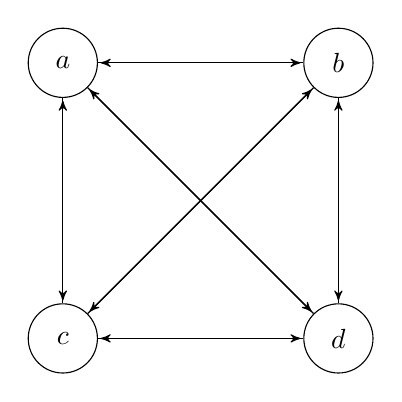
\begin{tikzpicture}[->,>=stealth',shorten >=1pt,auto,node distance=3.5cm,scale = 1,transform shape]

  \node[state] (a) [] {$a$};
  \node[state] (b) [right of=a] {$b$};
  \node[state] (c) [below of=a] {$c$};
  \node[state] (d) [below of=b] {$d$};

  \path (a) edge              node {} (b)
        (b) edge              node {} (a)
        (a) edge              node {} (c)
        (c) edge              node {} (a)
        (a) edge              node {} (d)
        (d) edge              node {} (a)
        (b) edge              node {} (c)
        (c) edge              node {} (b)
        (b) edge              node {} (d)
        (d) edge              node {} (b)
        (c) edge              node {} (d)
        (d) edge              node {} (c);

\end{tikzpicture}
\end{center}
Starting from vertex a, or any vertex to maintain generality, we can build a decision tree that traverses each path, this represents the the power set of the graph
\begin{center}
    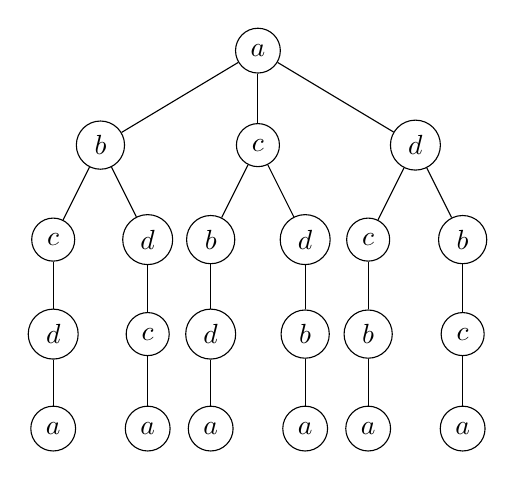
\begin{tikzpicture}[sibling distance=10em,
  every node/.style = {shape=circle, rounded corners,
    draw, align=center,
    top color=white, bottom color=white!5}, scale=0.8]
    \tikzstyle{level 1}=[sibling distance=25mm] 
    \tikzstyle{level 2}=[sibling distance=15mm] 
    \tikzstyle{level 3}=[sibling distance=10mm] 
    
  \node {$a$}
    child { node {$b$} 
        child {node {$c$}
        child {node {$d$}
        child {node {$a$}}}}
        child {node {$d$}
        child {node {$c$}
        child {node {$a$}}}}}
    child { node {$c$} 
        child {node {$b$}
        child {node {$d$}
        child {node {$a$}}}}
        child {node {$d$}
        child {node {$b$}
        child {node {$a$}}}}}
    child { node {$d$} 
        child {node {$c$}
        child {node {$b$}
        child {node {$a$}}}}
        child {node {$b$}
        child {node {$c$}
        child {node {$a$}}}}};
\end{tikzpicture}
\end{center}
The idea behind the exhaustive, brute-force approach is to traverse each path in the tree and then decide, this creates a very large problem to solve. The idea behind the dynamic approach is to start from the level 4 of the tree, which means we are now at the last vertex in the path and the next vertex from that completes the cycle and takes us back to the source node. This forms the smallest sub problem in the dynamic program. The next step would be go a level higher in the tree, which means we will now check the path length if we are reaching the source node from vertex $v$ and, we are reaching reaching vertex, $v$, from vertex, $u$ s.t. $u,v \in V$ where $V$ is the set of all vertices. We will keep doing this, and at each level we will decide the minimum path length of between n paths that are emerging from one vertex, this is done until the source node of the tree is reached, resulting in the minimum path. The dynamic algorithm can be generalised as a cost function, $g$, as follows:
$$g(i, S) = min_{k\in S} \bigg\{c_{ik} + g(k, S-\{k\})\bigg\}$$
s.t. $i$ is the source vertex, $S$ is the set of all vertices, $c_{ik}$ is the cost of going from some vertex $i$ to $k$. 
	

		
		
		
	\subsection{ Approximate Solutions}
		\subsubsection {Nearest Neighbour Algorithm}
		Nearest Neighbor is one of the approximate solutions to the problem of TSP that finds the cost of travelling from a point and returning back to the original point. To describe the problem in other words, a salesman starts from a city and visits the nearest unvisited city until they have been visited and returns back to the starting city. \newline \newline
		The algorithm is as follows: \newline
		Step 1.Choose any starting vertex. \newline
        Step 2.Whenever you reach any vertex, look at the weights of all the edges that lead to vertices you haven’t visited yet. Choose the one that has the least weight. \newline
        Step 3.Repeat step 2 until you’ve reached the last vertex. Else go back to the starting point.

 
		\subsubsection {Pairwise Exchange Method}
		\subsubsection {Christofides–Serdyukov Algorithm}
		
\section{Theoretical Runtime Analysis and Comparison}
\subsection{Nearest Neighbor}
Talking about the nearest neighbor, we can say that it is not optimal. This is because if we consider the brute-force approach, we get an accurate answer. Brute-force calculates the total cost of each Hamilton circuit and returns the minimum out of them. Hamilton circuit is a circuit where it travels to every vertex only once. As it can be seen that the cost of brute force gives us 23 whereas in nearest neighbor, even if we start from any vertex, we still end up with the cost that is greater than 23. However, nearest neighbor is efficient because it does not require to traverse through all the possible edges instead it uses the least weight whereas brute force calculates all possibilities taking n!. Nearest neighbor is $n^2$ because at each point, we need to find its nearest neighbor so that is n. And computing the distance from one point to all the other is n. So total is $O(n^2)$. \newline
\begin{figure}[htp]
    \centering
    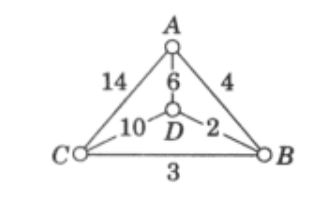
\includegraphics[width=5cm]{Graph.PNG}
    \label{fig:galaxy}
\end{figure} \newline
\textbf{Nearest Neighbor} \newline
\textbf{Start at A:} A, B, D, C, A. Total cost = 30 \newline
\textbf{Start at B:} B, D, A, C, B. Total cost = 25 \newline
\textbf{Start at C:} C, B, D, A, C. Total cost = 25 \newline
\textbf{Start at D:} D, B, C, A, D. Total cost = 25 \newline \newline
\textbf{Brute force} \newline
\textbf{Start at A:} A, B, C, D, A; Total cost = 23


\section{Empirical Runtime Analysis and Comparison}
Talking about the nearest neighbor algorithm, we see from the graph below that it runs extremely fast and is efficient as compared to the brute force algorithm. However, as mentioned earlier nearest neighbor is not optimal as it does not give us the accurate answer. The reason why the algorithm runs so fast is because it does not traverse over every path in the complete graph. However, it only traverses over those nodes which are not visited and have the least weight amongst them that are connected.
\begin{figure}[htp]
    \centering
    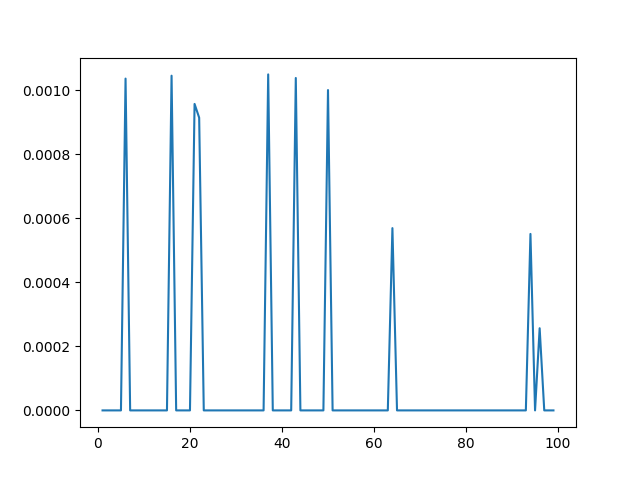
\includegraphics[width=5cm]{NN1fig2.png}
    \label{fig:galaxy}
\end{figure} \newline
\section{Conclusion}
\newpage
\section{References}
\begin{enumerate}
	\item \url{https://www.researchgate.net/publication/289195926_On_the_Nearest_Neighbor_Algorithms_for_the_Traveling_Salesman_Problem}
	\item \url{https://en.wikipedia.org/wiki/Travelling_salesman_problem#:~:text=The%20travelling%20salesman%20problem%20}
	\item Thomas H. Cormen, Charles E. Leiserson, Ronald L. Rivest, and Clifford Stein. 2009. Introduction to Algorithms, Third Edition (3rd. ed.)
	\item David L. Applegate, Robert E. Bixby, Vasek Chvatal, and William J. Cook. 2007. The Traveling Salesman Problem: A Computational Study. Princeton University Press, USA.
	\item\url{http://www.math.hawaii.edu/~les/m100/lecture9.pdf}
\end{enumerate}




\end{document}